\section{Durchführung}
\subsection{Verwendete Messinstrumente}
Damit der verwendete Aufbau richtig verstanden werden kann, müssen zunächst
einige wichtige Bauteile erläutert werden.
\subsubsection{Der Interferenzfilter}
Interferenzfilter werden verwendet, damit bestimmte Bereiche eines
kontinuierlichen Spektrums an Wellenlängen herausgefiltert werden können.
Verwendet wird eine dünne Schicht eines transparenten Dielektrikums, welches
von zwei semitransparenten Schichten umgeben ist. An diesen Schichten finden
eine Vielzahl von Reflektionen statt, welche interferieren. Um nur eine bestimmte
Wellenlänge zu erhalten, muss der Filter mit einigen Farbfiltern kombiniert
werden, die alle anderen Wellenlängen absorbieren. Da durch das Filtern einiges
an Intensität verloren geht wird dieser in diesem Experiment erst nach dem
Durchlaufen der Probe aufgebaut.

\subsubsection{Das Glan-Thompson Prisma}
In einem Glan-Thompson Prisma wird eine einfallende Welle in zwei senkrecht
zueinander polarisierten Teilstrahlen aufgespalten. Die beiden Strahlen
besitzen dabei zwei verschiedene Phasengeschwindigkeiten. Das Prinzip wird in
Abbildung \ref{fig:glan} dargestellt.

\begin{figure}[H]
  \centering
  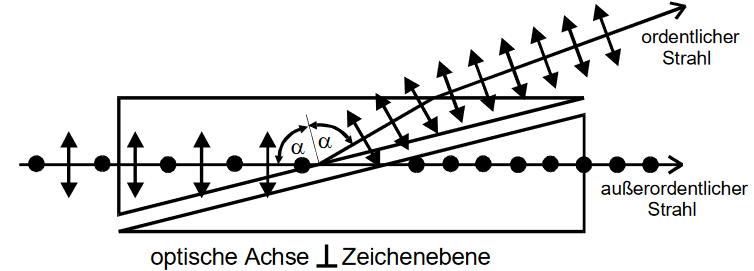
\includegraphics[width=12cm, height=4cm]{glanthom.png}
  \caption{Strahlengang einer Welle in einem Glan-Thompson Prisma}
  \label{fig:glan}
  \cite{skript}
\end{figure}

Der Kristall des Glan-Thompson Prismas ist doppelbrechend.
Für die räumliche Trennung der beiden Strahlen wird der Kristall diagonal
getrennt. Dann wird der Winkel $\alpha$ so gewählt, dass der ordentliche Strahl
eine Totalreflektion erfährt. Der außerordentliche Strahl wird jedoch nicht
total reflektiert. Das kann durch die verschiedenen Brechungsindizes begründet
werden. Der außerordentliche Strahl enthält nach Durchlaufen des Primas nur noch
eine Polarisationsrichtung. Das Prima wird somit benötigt um linar polarisierte
Stahlen zu erzeugen.

\subsection{Aufbau}
Der verwendete Aufbau ist in Abbildung \ref{fig:aufbau} dargestellt.

\begin{figure}[H]
  \centering
  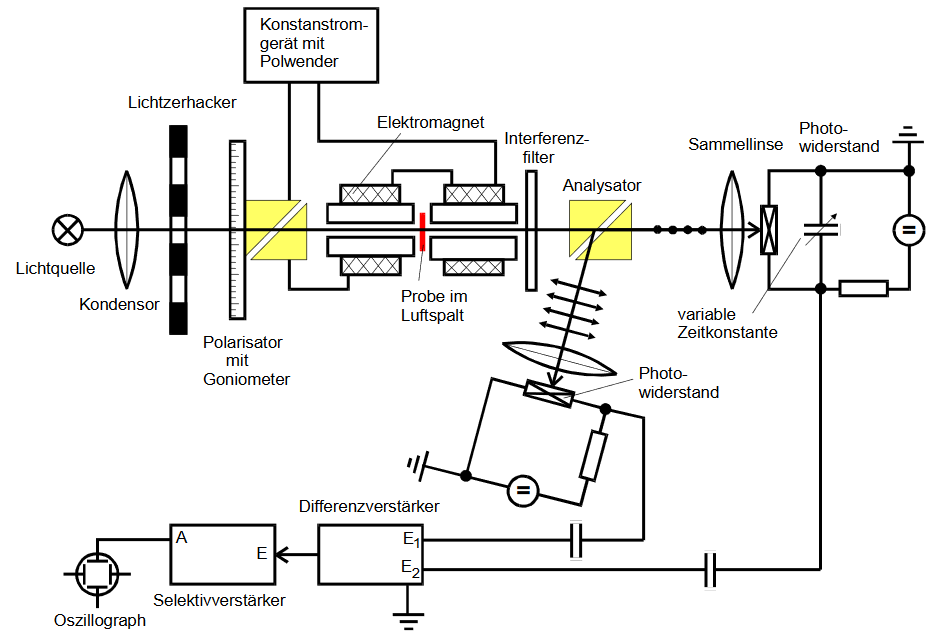
\includegraphics[width=14cm, height=10cm]{aufbau.png}
  \caption{Aufbau der im Versuch verwendeten Apparatur}
  \label{fig:aufbau}
  \cite{skript}
\end{figure}

Verwendet wird eine Halogen-Lampe mit einem Emissionsspektrum im Infrarotbereich.
Das Licht durchläuft zunächst eine Sammellinse, die es zu einem gebündelten
Strahl sammelt. Der Lichtzerhacker besteht aus einer rotierenden Sektorscheibe,
die das Licht in Impulse zerhackt. Die Methode die dadurch verwendet wird, wird
Wechsellichtmethode genannt. Sie wird verwendet, da die Photowiderstände auf
Grund ihres hohen Innenwiderstandes eine deutliche Rauschspannung produzieren.
Die Lichtimpulse treffen dann auf ein Glan-Thompson Prisma mit Goniometer, dass,
wie im Aufbau beschrieben, dazu dient, dass der Lichtstrahl linear polarisiert
in die Probe eintreten kann. Am Goniometer kann der Winkel $\theta$ eingestellt
und abgelesen werden. Das linear polarisierte Licht durchläuft dann das
Magnetfeld eines Elektromagneten in dessen Luftspalt die scheibenfömige
Probe eingeführt werden kann. Da der Luftspalt in dem Elektromagneten dazu führt,
dass keine komplette Homogenität des Magnetfeld entstehen kann, sollte die
Probe so klein wie möglich gewählt werden, also scheibenförmig. Der Elektromagnet
ist an einem Konstantstromgerät mit Polwender angeschlossen. Der Polwender dient
dazu, dass keine gefährlichen Induktionsspannungen beim Umpolen entstehen.
Nach Durchlaufen des Magnetfeldes wird das Licht in einem Interferenzfilter
monochromatisiert. In dem zweiten Glan-Thompson Prisma wird der Strahl dann
erneut in zwei senkrecht zueinander polarisierten Stahlen aufgeteilt. Die
Intensitäten beider Strahlen werden dann an zwei Photowiderständen gemessen.
Beide Spannungen werden dann auf einen Differenzverstärker gegeben. Die Spannung
verschwindet, wenn beide Strahlen in Betrag und Phase gleich sind. Von dort aus
wird die Spannung über einen Selektivverstärker, der mit der Frequenz vom
Lichtzerhacker abgestimmt ist, an ein Oszilloskop gegeben. Mit Hilfe des
Oszilloskop wird dann der Nullabgleich eingestellt. An dem Goniometer wird der
Winkel $\theta$ dann so geregelt, dass die Differenzspannung null ist. Dann wird
das Magnetfeld umgepolt und es wird erneut ein Nullabgleich vorgenommen. Dabei
müssen beide Winkel notiert werden.

\subsection{Die Justage}
Vor der Messung muss zunächst die Apperatur justiert werden. Dafür werden
zunächst die Probe und der Interferenzfilter aus dem Aufbau entfernt. Zunächst
muss die Funktionsweise der Polarisatoren geprüft werden, indem das Prisma so
eingestellt wird, dass die Lichtintensität für den durchgehenden Stahl
so gering wie möglich wird. Danach wird geprüft ob die gebündelten Strahlen
die Photodioden treffen. Der Lichtzerhacker wird dann auf eine Frequenz von
$\SI{500}{\hertz}$ eingestellt und der Selektivverstärker auf diese Frequenz
abgestimmt. Der Gütefaktor $Q$ wird dann auf einen Maximalwert eingestellt.
Da das Arbeiten mit maximaler Lichtintensität am sinnvollsten ist, wird der
Abstand zwischen Lampe, Linse und Zerhacker auf die maximale Intensität
ausgerichtet. Nach Einsetzen der Probe und des Interferenzfilters wird dann
geprüft, ob ein Nullabgleich erreicht werden kann. Dazu werden die Zeitkonstante
der Photowiderstände und die Stellung des Glan-Thompson Prismas variiert.

\subsection{Die Messung}
Im ersten Teil des Experiments soll die Kraftflussdichte $\text{B(z)}$ mit
Hilfe einer Hall-Sonde gemessen werden. Dazu wird der Feldstrom auf einen
Maximalwert geregelt. Mit der Sonde wird dann für bestimmte Weglängen $\text{x}$
der zugehörige Wert des Magnetfeldes aufgenommen. Dabei werden im Bereich des
Luftspaltes, in dem eigentlich die Probe steht, mehr Messwerte aufgenommen.
Danach wird die Faraday-Rotation für zwei n-dotierte und eine hochreine
Galliumarsenid Probe gemessen. Dazu werden jeweils acht verschiedene Filter
für jede Probenmessung verwendet. Bei der Faraday-Rotation wird für jede
Polung ein Nullabgleich geregelt und dann der Winkel $\theta$ notiert, sodass
bei jeder Probe bei jedem Filter zwei Winkel notiert werden.
